% \section{Introduction}
To get an approximation of the power consumption when configuring the GrAICore with a model and processing frames with it, we will provide calculations with energy parameters acquired from internal sources.

When configuring the GrAICore and processing an input frame, the major components that consume energy are as follows:
\begin{itemize}
    \item Configuration
    \begin{itemize}
        \item Reading data from the external memory
        \item Transferring data from the external memory to the config NoC
        \item Phits traversing (i.e., hops) through the config NoC
        \item Writing data to the neuron core's SRAM
    \end{itemize}
    \item Processing
    \begin{itemize}
        \item Processing the input frame by the model
    \end{itemize}
\end{itemize}

\section{Configuration energy}
Since we have access to various energy parameters for DDR memory, we will use DDR memory as an example.

\begin{figure}[hbtp]
    \centering
    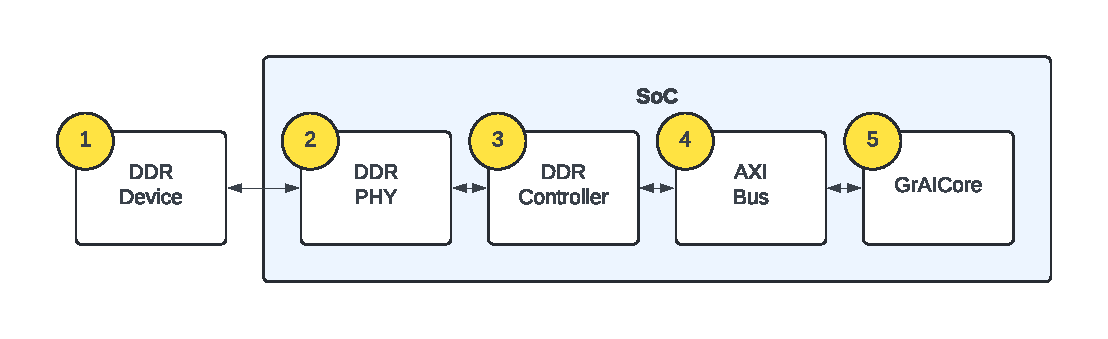
\includegraphics[width=0.8\linewidth]{assets/ddr_graicore_block_diagram.pdf}
    \caption{
        Interconnection of the DDR device and GrAICore
    }
    \label{fig:ddr_graicore_block_diagram}
\end{figure}

A typical system with DDR as external memory looks as shown in \cref{fig:ddr_graicore_block_diagram}.
% TODO add image
\begin{itemize}
    \item The \textit{DDR device} where the (model) data is read from.
    \item The \textit{DDR PHY} that connects the \textit{DDR device} and \textit{DDR controller}.
    \item The \textit{DDR controller} that handles the read/write requests from the \textit{GrAICore}.
    \item The \textit{AXI bus} that connects the \textit{DDR controller} and \textit{GrAICore}.
    \item The \textit{GrAICore} that transfers and writes data the SRAMs.
\end{itemize}

% It has been established that performing a hop on the Event NoC consumes around \SI{129}{fJ}.
% These hops are for phits of 32 bits.
% For the Config NoC (which uses phits of 16 bits), we are interested in the energy use for transferring phits of 16 bits. We can approximate this value by dividing the value for 32 phit hops into two. I.e., 129 fJ / 2 = 64.5 fJ. 

% Furthermore, it has been established that for the SRAM to write 64 bits, it consumes \SI{2.490}{pJ}.
% The SRAM system has the property to write 64 bits at once by first buffering four consecutive phits.
% This improves efficiency. 

For the analysis, we assume that we are using the newly proposed config NoC in \cref{sec:proposed_noc}. 
With the new packet format, a packet contains at most 65 data phits of 64 bits each.
That is, a maximum of 520 bytes\footnote{$65 \times \frac{\SI{64}{b}}{8} = \SI{520}{B}$} of payload per packet.
Furthermore, an additional injection point is introduced (see \cref{fig:segmentation_example_2}).
Next to the injection point connected to the router on the bottom left of the config NoC, a new one is added and connected to the router six positions up.

To estimate the energy cost for configuration, we require the following information from a model:
\begin{itemize}
    % \item Amount of data to read from the external memory
    \item Amount of data to write to the SRAMs
    \item Core destination of the data
\end{itemize}

The amount of data to write determines how much data will be read, transferred and written.
The location (specific neuron core) of the data determines the amount of hops the data has to perform in the config NoC.
The amount of data to write can also be used to determine the configuration time.
The configuration time is calculated by dividing the amount of data with the write bandwidth.
The configuration time is used for computing the energy for the \textit{DDR PHY}, \textit{DDR controller} and \textit{AXI bus}.

The amount of data to be written and to which neuron cores depends on several factors. % explain
Phits that needs to be transferred to neuron cores further away from an injection point will require more hops to reach, and therefore consume more energy than neuron cores closer to an injection point.
The amount of data that needs to be written to each core differs.
We can retrieve this information from the compiler.

For estimating the energy for the GrAICore component, we consider the config NoC and the SRAMs.
The config NoC consumes energy by transferring the data to its destinations.
The SRAM consumes energy by writing the data to its banks.
A single hop through the config NoC with a 64 bit phit consumes \SI{0.258}{pJ}.
% Writing back 64 bits to an SRAM consumes \SI{2.490}{pJ}.
Writing back 64 bits to an SRAM consumes \SI{4.980}{pJ}.

\begin{table}[hbtp]
\centering
\begin{tabular}{@{}lll@{}}
\toprule
\textbf{Component}      & \textbf{Usage}  &  \\
\midrule
DDR device              & \SI{0.11}{nJ/B} &  \\
DDR PHY                 & \SI{133}{mW}    &  \\
DDR controller          & ?               &  \\
AXI bus                 & \SI{80}{mW}     &  \\
NoC hop (\SI{64}{b})    & \SI{0.258}{pJ}  &  \\
SRAM write (\SI{64}{b}) & \SI{4.980}{pJ}  &  \\
\bottomrule
\end{tabular}
\caption{Energy parameters for each of the major energy consuming components. The shown power numbers for \textit{DDR PHY}, \textit{DDR controller} and \textit{AXI bus} are when at full capacity (i.e., best-case scenario).}
\label{tab:energy_parameters_ddr}
\end{table}

\subsection{Calculation}
The configuration energy consists of the reading, transferring and writing of data from the external memory to the GrAICore's SRAMs. 

Let $C$ be the set of tuples holding the coordinates of every core:
\begin{equation*}
    C = \{\,\left(x,y\right) \in \mathbb{N}^2 \mid 1 \leq x \leq 12 \wedge 0 \leq y \leq 11 \,\} 
\end{equation*}

Notice that the x-coordinate and y-coordinate starts at index $1$ and $0$ respectively.

\Cref{fig:model_data_heapmap} shows for a $80\%$ pruned version of ResNet-50\footnote{Internally named \texttt{resnet50\_pruned80\_star}} the amount of data that needs to be written to each of the 144 neuron cores.
We observe that the data is not uniformly distributed across the SRAMs.
Therefore, we require information how much data needs to be transferred to each SRAM.

\begin{figure}[hbtp]
    \centering
    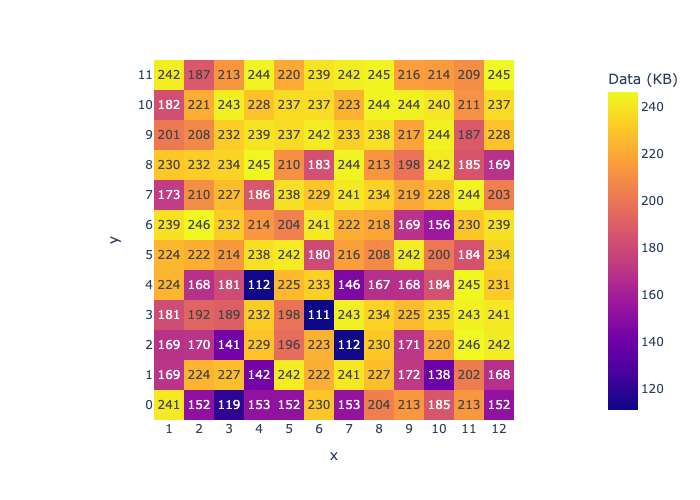
\includegraphics[width=0.8\linewidth]{assets/model_data_heatmap.png}
    \caption{Amount of data to be written to each core for the ResNet-50 model (80\% pruned).}
    \label{fig:model_data_heapmap}
\end{figure}

Let $D$ be a matrix of $12 \times 13$ with $D_{i,j}$ denoting the amount of bytes to be written to core $\left( i,j \right)$.
$D$ has an additional column due to the x-coordinates not starting from index $0$.
Its left-most column is unused (i.e., $D_{0,0}, D_{0,1}, \cdots, D_{0,11}$).
This matrix can be constructed from the artifacts outputted by the compiler.

The number of phits to be transferred through the config NoC influences the total energy costs.
In particular, the amount of phits to be transferred affects the number of hops to be taken in total and the amount of data to be written to the SRAMs.
Therefore, we need to determine how many phits needs to be transferred to each neuron core.
% The number of phits to be transferred influences the energy cost in the config NoC hops and SRAM writes.
% A packet can contain up to 520 bytes\footnote{$65 \times \frac{64}{8}$} of payload data. 
A packet can contain up to 65 data phits, that is $65 \times \SI{64}{b} = \SI{520}{B}$ of payload data.
% If we transfe
Suppose we need to transfer $d$ bytes to a neuron core, we then require a total of $\left\lfloor \frac{d}{520} \right\rfloor$ packets with 65 data phits.
% If $d \bmod 520 > 0$, then there is an additional packet consisting of $\left\lceil \frac{\left( d \bmod 520 \right) \times 8}{64}\right\rceil$ data phits.
If $\left( d \bmod 520 \right) > 0$, then there is an additional packet for the remaining $\left( d \bmod 520 \right)$ bytes of data.
The remaining packet will consist of $\left\lceil \frac{d \bmod 520}{8}\right\rceil$ data phits.
Note that each packet also contains a single phit of 64 bits for the header information.


The total energy cost for configuring the GrAICore can be estimated with the following equation:
\begin{equation}
    E_{\textrm{config}} = E_{\textrm{ext\_mem}} + E_{\textrm{noc}} + E_{\textrm{write}}
\end{equation}

With:
\begin{align*} 
E_{\textrm{ext\_mem}} &= 
        \sum_{c \in C}^{}{E_\textrm{read\_ext\_mem}(D_c) + E_{\textrm{send\_to\_noc}}(D_c)} \\
E_{\textrm{noc}} &=
    E_{\textrm{hop}} \times \sum_{c \in C}^{}{N_\textrm{hops}(c) \times p_{\textrm{total}}(D_c)} \\
E_{\textrm{write}} &=
    E_{\textrm{sram\_write\_64b}} \times \sum_{c \in C}^{}{p_{\textrm{data}}(D_c)}
\end{align*}

And:
\begin{align*} 
N_{\textrm{hops}}(x,y) &=
    \begin{cases} 
        x + y & \textrm{if } 0 \leq y \leq 5 \\
        x + y - 6 & \text{if } 6 \leq y \leq 11
    \end{cases}
\\
p_{\textrm{total}}(d) &=
    \left\lfloor \frac{d}{520} \right\rfloor \times (65 + 1) + \left\lceil \frac{d \bmod 520}{8} \right\rceil + 1 =
    \left\lceil \frac{d}{8} \right\rceil + \left\lfloor \frac{d}{520} \right\rfloor + 1 
\\
p_{\textrm{data}}(d) &=
    \left\lfloor \frac{d}{520} \right\rfloor \times 65 + \left\lceil \frac{d \bmod 520}{8} \right\rceil =
    \left\lceil \frac{d}{8} \right\rceil
\end{align*}

\begin{eqexpl}[15mm]
    \item{$p_{\textrm{total}}(D_c)$} total phits (includes headers) for transferring $D_c$ bytes
    \item{$p_{\textrm{data}}(D_c)$} total data phits (excludes headers) for transferring $D_c$ bytes
    \item{$N_{\textrm{hops}}(c)$} the amount of hops required to reach a neuron core at coordinate $c$, starting from the router closest to the injection point. It has two sub-functions due to the new config NoC's dual injector architecture
    \item{$E_{\textrm{read\_ext\_mem}}(D_c)$} energy for reading $D_c$ bytes from the external memory
    \item{$E_{\textrm{send\_to\_noc}}(D_c)$} energy for sending $D_c$ bytes from the external memory to the config NoC
    \item{$E_{\textrm{hop}}$} energy for performing a single hop in the config NoC
    \item{$E_{\textrm{sram\_write\_64b}}$} energy for writing back 64 bits to a neuron core's SRAM
\end{eqexpl}

\section{Processing energy}
The processing energy is the energy consumed when the GrAICore is processing input frames.
% Note that the GrAICore does not make use of the config NoC to process input frames.
Note that the GrAICore uses the event NoC for communication between nodes when processing input frames, the config NoC is not involved in this process.

The processing energy can be estimated with the following equation:
\begin{equation}
    E_{\textrm{frame}} = \textrm{avg\_util} \times \textrm{cores\_used} \times \textrm{processing\_latency} \times \SI{21}{mW}
\end{equation}

These parameters can be obtained by simulating the model with \textit{GrAIPEFRUIT}, an in-house simulator for estimating inference performance.
Processing latency (\textrm{processing\_latency}) is the time the model takes to fully process a single frame, from input to output.
Cores used (\textrm{cores\_used}) is the amount of neuron cores that were used to execute the model.
Average utilization (\textrm{avg\_util}) is the average percentage of the time the cores were active while the frame was processed. 
The constant \SI{21}{mW} is the approximated power usage of a single neuron core while it's being fully utilized.
This constant is obtained from RTL simulations.

Since the config NoC is not involved in the processing of an input frame, any change to the config NoC does not influence the processing energy.
A significant factor (other than hardware changes) that may affect the processing energy is the mapping performed by the compiler on the original model. 
Different mappings on the same model have an effect on the average utilization and the number of neuron cores used, which in turn influences the processing latency.

\section{Evaluation}
The energy to configure the system is mainly dependent on the amount of data that is to be transferred.
% Since every model has a different size, we calculate the energy costs individually.



\lipsum[1]

We calculate the energy consumption for writing various models and processing it with an input frame.

We look at the following models
% Please add the following required packages to your document preamble:
% \usepackage{booktabs}
\begin{table}[]
\centering
\begin{tabular}{@{}lrrrrr@{}}
\toprule
\textbf{Model name}                                  & \textbf{\begin{tabular}[c]{@{}l@{}}Latency\\ (ms)\end{tabular}} & \textbf{Cores} & \textbf{Avg util.} & \textbf{\begin{tabular}[c]{@{}l@{}}To write\\ (MiB)\end{tabular}} & \textbf{\begin{tabular}[c]{@{}l@{}}Time to \\ configure (ms)\end{tabular}} \\ \midrule
% efficientnet (16b)                                   & 1.590                                                           & 144            & 52.11\%            & 21.09                                                             & 1.728                                                                      \\
efficientnet (8b)                                    & 1.642                                                           & 144            & 50.89\%            & 16.15                                                             & 1.323                                                                      \\
% mobnetv2 (16b)                                       & 1.293                                                           & 144            & 40.96\%            & 14.27                                                             & 1.169                                                                      \\
mobnetv2 (8b)                                        & 1.296                                                           & 144            & 40.78\%            & 10.67                                                             & 0.874                                                                      \\
hand\_tracker\_star\_v2                              & 1.480                                                           & 144            & 36.62\%            & 12.33                                                             & 1.010                                                                      \\
hand\_detector (8b)                                  & 4.809                                                           & 144            & 68.03\%            & 19.12                                                             & 1.566                                                                      \\
% hand\_models\_combined\_tracker\_star\_v2 (source 0) & 5.629                                                           & 144            & 47.20\%            & 23.26                                                             & 1.905                                                                      \\
% hand\_models\_combined\_tracker\_star\_v2 (source 1) & 1.476                                                           & 144            & 37.09\%            & 23.26                                                             & 1.905                                                                      \\
% hand\_models\_combined\_tracker\_star\_v2 (both)     & 7.105                                                           & \#N/A          & \#N/A              & 23.26                                                             & 1.905                                                                      \\
resnet50\_p0                                         & 5.136                                                           & 144            & 37.98\%            & 23.45                                                             & 1.921                                                                      \\
resnet50\_p1                                         & 1.320                                                           & 143            & 36.44\%            & 7.37                                                              & 0.604                                                                      \\
resnet50                                             & 5.765                                                           & 144            & 36.35\%            & 29.58                                                             & 2.424                                                                      \\
resnet101\_p0                                        & 7.080                                                           & 144            & 33.40\%            & 28.75                                                             & 2.356                                                                      \\
resnet101\_p1                                        & 2.647                                                           & 143            & 36.42\%            & 20.06                                                             & 1.644                                                                      \\
resnet101\_p2                                        & 4.011                                                           & 144            & 33.12\%            & 30.44                                                             & 2.494                                                                      \\
resnet101\_p3                                        & 2.343                                                           & 143            & 33.55\%            & 17.71                                                             & 1.451                                                                      \\
resnet101\_p4                                        & 2.040                                                           & 143            & 26.19\%            & 15.54                                                             & 1.273                                                                      \\
resnet101*                                           & 18.121                                                          & ---            & ---                & 112.51                                                            & 9.218                                                                      \\
resnet101\_pruned\_p0                                & 6.552                                                           & 144            & 38.10\%            & 15.87                                                             & 1.300                                                                      \\
resnet101\_pruned\_p1                                & 3.245                                                           & 143            & 34.31\%            & 10.43                                                             & 0.855                                                                      \\
resnet101\_pruned\_p2                                & 4.501                                                           & 143            & 33.83\%            & 16.00                                                             & 1.311                                                                      \\
resnet101\_pruned\_p3                                & 2.114                                                           & 143            & 38.08\%            & 10.22                                                             & 0.838                                                                      \\
resnet101\_pruned\_p4                                & 2.437                                                           & 143            & 24.25\%            & 7.69                                                              & 0.630                                                                      \\
resnet101\_pruned*                                   & 18.849                                                          & ---            & ---                & 60.22                                                             & 4.934                                                                      \\
\bottomrule
\end{tabular}
\caption{}
\label{tab:my-table}
\end{table}
